\documentclass[runningheads]{llncs}

\usepackage[T1]{fontenc}
\usepackage{amsmath}
\usepackage{amssymb}
\usepackage{multirow}
\usepackage{graphicx}
\usepackage{booktabs}      % \toprule, \midrule, \bottomrule
\usepackage{marvosym}      % \Letter (in author block)
\usepackage{hyperref}      % \url
\usepackage{pifont}        % \ding{51} / \ding{55}
\usepackage{colortbl}      % \rowcolor
\usepackage{xcolor}        % gray!15 color spec

\begin{document}

\title{In-Network IoT Attack Detection Using Principal Component Analysis and Machine Learning Models on P4 Programmable Data Planes}
\titlerunning{In-Network IoT Attack Detection Using PCA and ML Models on P4}

\author{
Viet Anh Phan\inst{1}\orcidID{0009-0003-1787-8063}\textsuperscript{\Letter} \and
Mingyu Ma\inst{2,4}\orcidID{0009-0005-7045-4096} \and 
Tung V. Doan\inst{2,4} \and
Giang T. Nguyen\inst{2,4}\orcidID{0000-0001-7008-1537} \and \\
Frank H.P. Fitzek\inst{3,4}\orcidID{0000-0001-8469-9573} \and
Jan Jerabek\inst{1}\orcidID{0000-0001-9487-5024} \and 
Lukas Malina\inst{1}\orcidID{0000-0002-7208-2514} \and
Jiri Hosek\inst{1}\orcidID{0000-0002-8382-9185}
}

\authorrunning{Phan et al.}

\institute{
Department of Telecommunications,
Brno University of Technology, Czech Republic \\
\email{\{243760, jerabekj, malina, hosek\}@vut.cz}
\and
Haptic Communication Systems, TU Dresden, Germany \\
\and
Deutsche Telekom Chair of Communication Networks, TU Dresden, Germany \\
\and
Centre for Tactile Internet with Human-in-the-Loop (CeTI), TU Dresden, Germany
\email{\{mingyu.ma, tung.doan\_van, giang.nguyen, frank.fitzek\}@tu-dresden.de}
}

\maketitle
\begin{abstract}
IoT gateways are vital to the scalability and security of IoT networks. P4 programmable switches let these gateways parse, track, and classify traffic directly in the forwarding pipeline at line rate, avoiding the latency and bandwidth cost of offloading detection to an external controller or server. Tree-based models that detect malicious IoT traffic already run entirely in this pipeline, but dimensionality reduction via Principal Component Analysis (PCA) has so far been deployed as a standalone module, never integrated with the downstream model under a single range-match encoding. This calls for an integrated solution. This paper presents the first P4 intrusion-detection pipeline that combines PCA projection and tree-based attack detection under a single range-match abstraction, evaluated on a Raspberry Pi~4 running BMv2 (\texttt{simple\_switch\_grpc}). Across $32$ deployed configurations (Decision Tree and 4-tree Random Forest, with and without PCA), the raw range-match model achieves the highest in-distribution macro F1 on CIC-IoT 2023 ($98.47\%$) but degrades to $15.57\%$ on a disjoint Mu-IoT capture, as the model fails to generalize to the new traffic distribution. The recommended PCA $+$ Decision Tree at $k{=}7$ achieves $95.79\%$ macro F1 in distribution and $48.31\%$ on the disjoint capture, a $32.74$ percentage-point cross-dataset gain at the cost of only $2.68$ percentage points in distribution, making strong in-distribution accuracy and cross-dataset robustness jointly attainable. The recommended operating point clears the Tofino-1 per-stage match-key budget; stage-count compaction is the identified path to full Tofino-1 deployment.


\keywords{P4 programmable data plane \and In-network machine learning \and IoT \and Intrusion detection system \and Principal Component Analysis \and Decision tree \and Random forest \and Range match tables \and Bidirectional flow features \and Line-rate classification}
\end{abstract}
%
%
%
\section{Introduction}\label{sec:intro}
The Internet of Things (IoT) connects an increasing number of resource-con\-strained devices through gateway switches that aggregate heterogeneous traffic before it enters the wider network. These gateways are a natural defensive vantage point because every flow from the protected segment passes through them, and they are also a critical bottleneck: an intrusion-detection system (IDS) that mirrors traffic off the forwarding path, or delegates the classification decision to an external controller, introduces latency and bandwidth overhead that traditional middlebox and SDN deployments cannot eliminate~\cite{Gao2021,Wang20241480}. P4 programmable data planes lift this restriction by letting the switch parse, track, and classify flows in the pipeline at line rate, without recirculation or controller round trips. In-network ML detection has therefore become an active research area~\cite{Xiong201925,Lee202523143,Zheng20242,Akem2024}.

The same pipeline must run on two very different targets. At the IoT-gateway tier, P4 has reached small-footprint hardware through P4Pi~\cite{Laki2021p4pi}, a Raspberry-Pi-based BMv2 platform on which P4Pir~\cite{Zang20249244} has shown that DT and RF classifiers are feasible. All experiments in this paper are conducted on the same platform tier, a Raspberry Pi~4 running BMv2 (\texttt{simple\_switch\_grpc}) with the v1model architecture. At higher tiers, where industrial IoT and cyber-physical workloads require deterministic latency, programmable ASICs such as Intel Tofino are the target~\cite{Akem2024}. Both tiers expose the same constraint: limited on-chip memory and a fixed number of pipeline stages restrict how expressive the classifier can be, so a P4 IDS pipeline that scales gracefully must keep its match-action footprint small.

Despite this progress, the existing body of work reveals five persistent gaps. \emph{First}, most in-network ML systems rely on exact-match encoding, where the classifier table stores one entry per unique discretized training feature vector~\cite{Lee202523143,Zheng20242,Zheng20242555}. Coverage is therefore restricted to feature combinations actually observed during training, and the number of entries scales with the granularity of the discretization grid and the size of the training set $N$, so adding training samples or refining feature granularity grows the table proportionally and stresses on-chip memory budgets~\cite{Bosshart2013}. \emph{Second}, the majority of P4-based detection systems perform only binary classification, which limits their utility for security teams that must triage diverse threats. \emph{Third}, extracting bidirectional flow statistics entirely in the data plane remains underexplored; most systems rely on unidirectional or packet-level features, or offload feature computation to an external server. \emph{Fourth}, dimensionality reduction has been treated in isolation from the downstream classifier: although Planter~\cite{Zheng20242} supports PCA as a standalone module, no prior work integrates PCA with a downstream classifier under a single range-match encoding, and no prior work makes the trade-off between a raw-feature classifier and a PCA-projected one explicit on hardware-relevant axes (per-entry match-key width, classifier-table size, and pipeline-stage placement). \emph{Fifth}, translating a trained ML model into a deployable P4 program typically requires significant manual effort across separate tools for training, feature selection, table generation, and code synthesis.

This paper addresses all five gaps through the following contributions:

\begin{itemize}
    \item PCA is integrated as a dimensionality-reduction stage that is itself encoded as range-match P4 tables and feeds the downstream classifier through the same encoding. To the best of the authors' knowledge, this is the first integration of PCA with a downstream classifier under a single range-match encoding in a P4 data plane. The trade-off introduced by this stage is characterized in detail: PCA exposes a tunable match-key dial via $k$ (from $32$ bits at $k{=}1$ up to $480$ bits at $k{=}15$, versus the $256$-bit raw composite key) and improves cross-dataset robustness, at the cost of roughly $2$ times more classifier entries than the raw-feature pipeline.
    \item DT and RF classifiers are deployed as range-match P4 entries rather than exact-match entries, representing each tree leaf as a single rule with per-feature ranges. This naturally expresses the axis-aligned splits of a decision tree and yields the strongest in-distribution operating point of the pipeline (raw range-match DT, macro F1 $98.47\%$, $5\,119$ entries on CIC-IoT 2023).
    \item Multiclass classification is performed directly in the data plane on the CIC-IoT 2023 dataset~\cite{Neto2023} (Benign, DoS, Brute Force, Reconnaissance), in contrast to the predominantly binary detectors in prior work~\cite{Ilha20213121,Musumeci2022,Lee202523143}.
    \item The pipeline extracts $18$ bidirectional flow features in the data plane across six categories (protocol, ports, timing, volume, TCP flags, TCP window), substantially richer than the unidirectional or packet-level features used by prior in-network approaches~\cite{Nguyen2024,Akem2024,Zang20249244}.
    \item An automated end-to-end pipeline is provided that covers feature extraction, model training, optional PCA projection, table-entry generation, and P4 code synthesis, deployed and evaluated on a Raspberry Pi~4, including a \emph{cross-dataset} transfer (from CIC-IoT 2023 to Mu-IoT) to quantify how each encoding generalizes beyond its training distribution.
\end{itemize}

The full source code, training pipeline, and table-generation scripts used in this paper are publicly available at \url{https://github.com/vafekt/p4sec}.

\section{Related Work}\label{sec:related}
Prior work is analyzed along five dimensions: inference location, table encoding, feature extraction, classification granularity, and use of dimensionality reduction. Table~\ref{tab:comparison} provides the structured comparison.

\textbf{In-network ML inference:} Xiong and Zilberman~\cite{Xiong201925} first mapped DT, SVM, Naive Bayes, and K-means to match-action tables on BMv2 and NetFPGA SUME with a small set of packet-level features. IIsy~\cite{Zheng20242555} added a hybrid Tofino architecture forwarding low-confidence packets to a backend; its discretized-feature encoding allocates one entry per discretized value, so table sizes scale with the number of distinct feature values. Planter~\cite{Zheng20242} unified eleven ML algorithms under three mapping methodologies (direct, encode-based, and lookup) and includes PCA as a standalone module. As an ML-mapping framework it does not include a feature-extraction stage; it consumes pre-computed CSV features and does not integrate PCA with a downstream classifier under a single range-match encoding. SwitchTree~\cite{Lee202523143} placed an RF of three trees in BMv2 with exact-match direct mapping (binary only on UNSW-NB15), Akem et al.~\cite{Akem2024} encoded RF on Tofino for encrypted-traffic classification with range/ternary entries, and Zang et al.~\cite{Zang20249244} deployed DT/RF on IoT gateways through Planter using network-, transport-, and application-layer fields for binary detection. Ganesan and Sarac~\cite{Ganesan2025} use range encoding for an ensemble on CIC-IDS2017 but only for binary classification, while attack-specific statistical approaches~\cite{Ilha20213121,Wang20241480,Li2024} rely on hand-tuned thresholds rather than learned boundaries. Hybrid systems~\cite{El-Sayed2025,Musumeci2022,Doriguzzi-Corin2024} extract features in the data plane but run inference in the controller, reintroducing the latency that in-network processing aims to eliminate.

\textbf{Encoding and dimensionality reduction:} Exact-match encoding~\cite{Lee202523143,Zheng20242} requires one entry per discretized value and scales with the discretization grid; range/ternary encoding~\cite{Akem2024,Ganesan2025,Zheng20242} collapses contiguous intervals into single rules by exploiting axis-aligned tree splits. The proposed pipeline is the first to adopt range match for both the PCA projection and the downstream classifier, yielding a compact $5\,119$-entry raw DT and a tunable PCA ladder ($k\!\in\!\{1,\dots,15\}$) under a single encoding. Range and exact match consume different on-chip resources on programmable ASICs (range tables compile to TCAM after prefix expansion, while exact-match tables are placed in SRAM hash banks), so the entry-count comparison is on the logical rule set, not a direct TCAM saving over exact match.

\begin{table}[t]
\centering
\caption{Comparison of P4 based ML approaches. DP = Data Plane, Hy = Hybrid, B = Binary, M = Multiclass. DP~Red. = in-data-plane dimensionality reduction.}
\label{tab:comparison}
\renewcommand{\arraystretch}{1.15}
\setlength{\tabcolsep}{3pt}
\begin{tabular}{l c c c c c}
\toprule
\textbf{Work} & \textbf{Inference} & \textbf{Match Type} & \textbf{Bidir.\ Flow} & \textbf{Classes} & \textbf{DP~Red.} \\
\midrule
Xiong~\cite{Xiong201925}          & DP & Exact/Ternary & \ding{55} & M & \ding{55} \\
IIsy~\cite{Zheng20242555}         & Hy & Exact/Ternary & \ding{55} & B & \ding{55} \\
Planter~\cite{Zheng20242}         & DP & Exact/Ternary & \ding{55} & M & PCA\textsuperscript{a} \\
Euclid~\cite{Ilha20213121}        & DP & Ternary       & \ding{55} & B & \ding{55} \\
CD2P~\cite{Wang20241480}          & Hy & Not applied   & \ding{55} & B & \ding{55} \\
HISTA~\cite{Li2024}               & Hy & Not applied   & \ding{55} & B & \ding{55} \\
CO-STOP~\cite{El-Sayed2025}       & Hy & Not applied   & \ding{55} & M & \ding{55} \\
Musumeci~\cite{Musumeci2022}      & Hy & Not applied   & \ding{55} & B & \ding{55} \\
SwitchTree~\cite{Lee202523143}    & DP & Exact         & \ding{51} & B & \ding{55} \\
Akem~\cite{Akem2024}              & DP & Ternary/Range & \ding{55} & M & \ding{55} \\
P4DDLe~\cite{Doriguzzi-Corin2024} & Hy & Exact         & \ding{51} & B & \ding{55} \\
P4Pir~\cite{Zang20249244}         & DP & Exact         & \ding{55} & B & \ding{55} \\
Ganesan~\cite{Ganesan2025}        & DP & Range         & \ding{55} & B & \ding{55} \\
\midrule
\rowcolor{gray!15}
\textbf{Ours} & \textbf{DP} & \textbf{Range} & \ding{51} & \textbf{M} & \textbf{PCA\textsuperscript{b}} \\
\bottomrule
\multicolumn{6}{l}{\textsuperscript{a}Standalone module, not integrated with classifier.} \\
\multicolumn{6}{l}{\textsuperscript{b}Integrated with downstream classifier via range match.} \\
\end{tabular}
\end{table}

As Table~\ref{tab:comparison} illustrates, no existing work simultaneously combines range-match PCA encoding, range-match tree classifiers, multiclass output with four or more classes, bidirectional flow features, and a fully automated PCAP-to-P4 pipeline. Planter~\cite{Zheng20242} is the closest prior work, but the differences matter in practice: it treats PCA as a standalone module and uses an exact-match-based mapping for its tree classifier in the configuration most directly comparable to the proposed design, so its table size scales with the number of distinct discretized feature values, whereas the proposed pipeline encodes \emph{both} the PCA projection and the downstream tree classifier as range-match entries, representing each tree leaf as one rule with per-feature ranges.

\section{Proposed Framework}\label{sec:framework}

The system operates in two phases. An \emph{offline training phase} (Fig.~\ref{fig:pipeline}) processes labeled captures into a compiled P4 program and pre-populated table entries; an \emph{online inference phase} (Fig.~\ref{fig:framework}) then executes feature extraction, dimensionality reduction, and classification entirely in the data plane at line rate. Both phases use identical fixed-point arithmetic, so the switch reproduces the offline classifier's predictions modulo the $b$-bit rounding of the quantized PCA codes (Section~\ref{sec:pipeline}, Step~2).

\begin{figure}[!t]
\centering
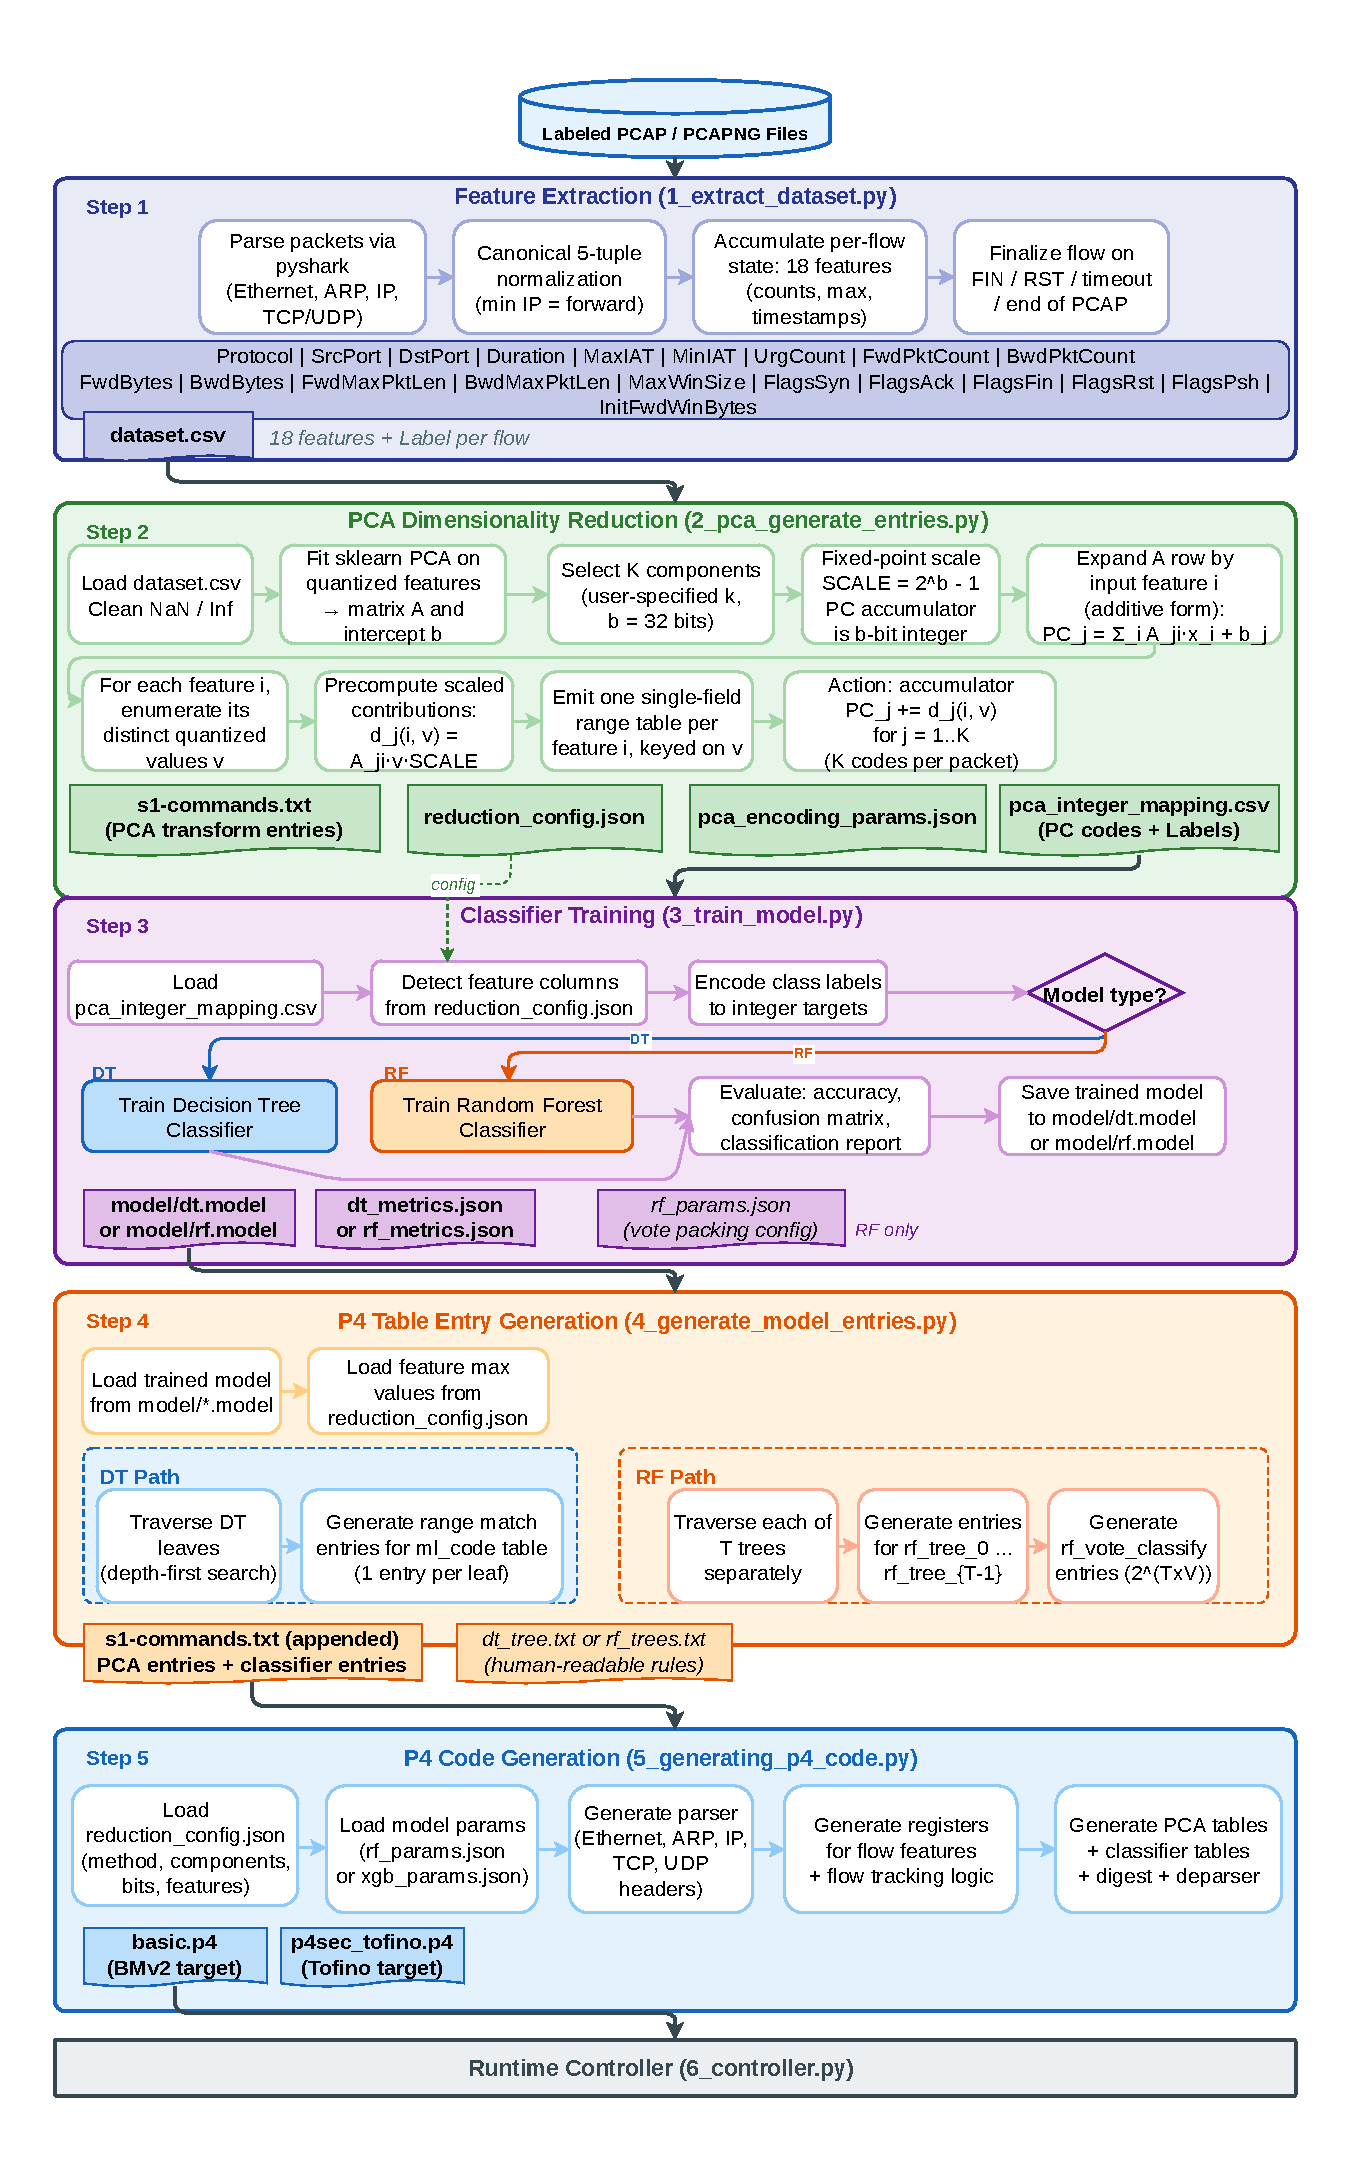
\includegraphics[width=0.7\columnwidth]{images/offline_pipeline.pdf}
\caption{Offline training pipeline. Five offline stages convert raw PCAPs into a compiled P4 program with pre-populated range-match tables for the additive PCA projection and the downstream classifier.}
\label{fig:pipeline}
\end{figure}

\begin{figure}[!ht]
\centering
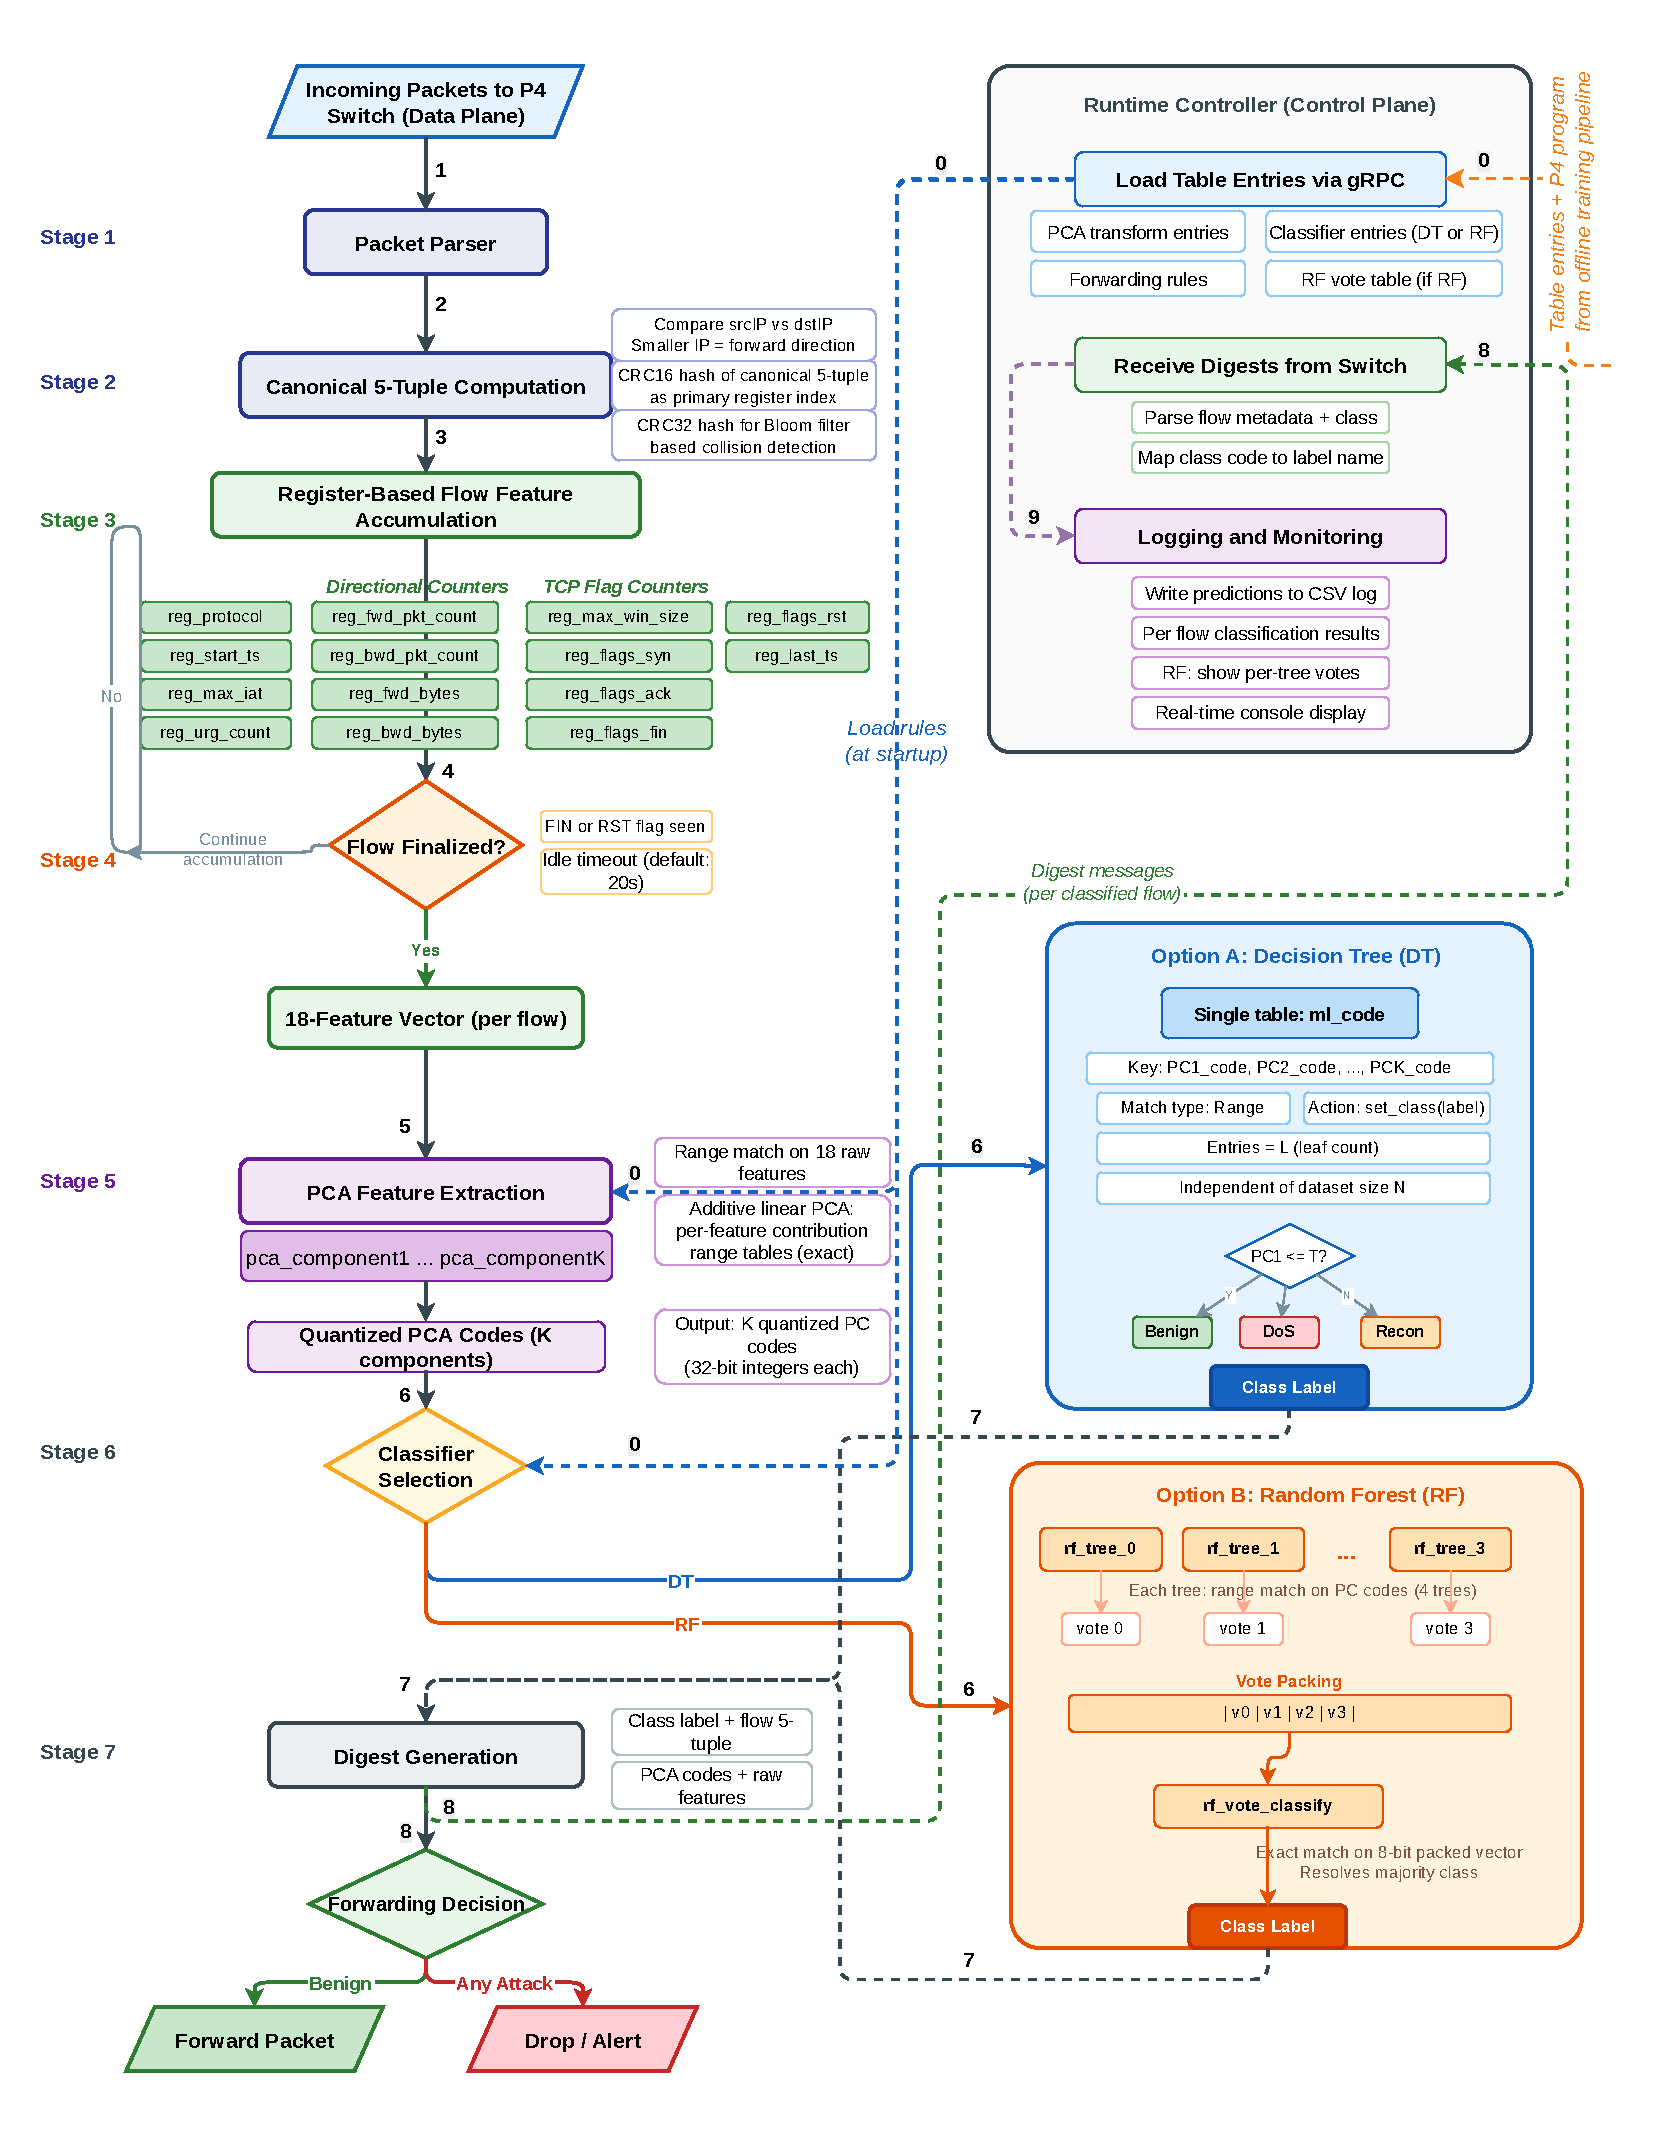
\includegraphics[width=0.7\columnwidth]{images/Framework.pdf}
\caption{In-network inference pipeline. Each finalized flow is canonicalized, accumulated into $18$ bidirectional flow features, projected through the additive PCA range tables into $K$ quantized codes, classified by a Decision Tree or 4-tree Random Forest, and emitted as a digest to the controller.}
\label{fig:framework}
\end{figure}

%──────────────────────────────────────────────────────────────────────
\subsection{Offline Training Phase}\label{sec:pipeline}
%──────────────────────────────────────────────────────────────────────

The offline pipeline (Fig.~\ref{fig:pipeline}) transforms raw PCAP captures into a compiled P4 program and a set of table-entry commands. The training data is drawn from \mbox{CIC-IoT 2023}~\cite{Neto2023}, a recent benchmark generated on a physical testbed covering IoT attacks across seven categories, which provides raw PCAPs (required for header-level compilation). The pipeline comprises five steps, each implemented as a standalone Python script.

\noindent\textbf{Step~1: Feature extraction}

Raw PCAP files are parsed to extract bidirectional flow features into a CSV dataset. Each flow is identified by a canonical five-tuple in which the endpoint with the numerically smaller IP address is the forward source; the same normalization is replicated in the generated P4 code. A CRC16 hash indexes the per-flow register arrays; a CRC32 hash indexes a Bloom-filter register for collision detection. A flow is finalized on a TCP FIN or RST flag, or after an idle timeout of $20$\,s; only finalized flows proceed to classification. Table~\ref{tab:features} lists the $18$ features produced.

\begin{table}[!t]
\centering
\caption{Eighteen bidirectional flow features extracted in the data plane, grouped by category. The \textbf{Bits} column lists the quantized width used by the deployed P4 classifier; the per-feature widths sum to $256$ bits (the raw range-match DT match-key width).}
\label{tab:features}
\renewcommand{\arraystretch}{1.1}
\setlength{\tabcolsep}{4pt}
\begin{tabular}{lllc}
\toprule
\textbf{Category} & \textbf{Feature} & \textbf{Description} & \textbf{Bits} \\
\midrule
Protocol  & Protocol         & IP protocol (TCP/UDP/ICMP)         & 8  \\
\midrule
\multirow{2}{*}{Ports}
          & SrcPort          & Canonical source port              & 16 \\
          & DstPort          & Canonical destination port         & 16 \\
\midrule
\multirow{2}{*}{Timing}
          & Duration         & First-to-last packet time          & 16 \\
          & MaxIAT           & Maximum inter-arrival time         & 16 \\
\midrule
\multirow{6}{*}{Volume}
          & FwdPktCount      & Forward packet count               & 16 \\
          & BwdPktCount      & Backward packet count              & 16 \\
          & FwdBytes         & Forward byte count                 & 16 \\
          & BwdBytes         & Backward byte count                & 16 \\
          & FwdMaxPktLen     & Max forward packet length          & 16 \\
          & BwdMaxPktLen     & Max backward packet length         & 16 \\
\midrule
\multirow{5}{*}{TCP Flags}
          & FlagsSyn         & SYN packet count                   & 8  \\
          & FlagsAck         & ACK packet count                   & 16 \\
          & FlagsFin         & FIN packet count                   & 8  \\
          & FlagsRst         & RST packet count                   & 8  \\
          & FlagsPsh         & PSH packet count                   & 16 \\
\midrule
\multirow{2}{*}{Window}
          & MaxWinSize       & Maximum TCP window size            & 16 \\
          & InitFwdWinBytes  & Initial forward TCP window         & 16 \\
\bottomrule
\end{tabular}
\end{table}


The features align with the flow-level statistics used by Zeek~\cite{Paxson1998} and NetFlow/IPFIX~\cite{Hofstede20142037}; separating forward and backward counters exposes the directional asymmetries that characterize flood, scan, and amplification attacks. Flag counters and window-size extrema target TCP control-plane patterns dominant in CIC-IoT 2023; volume, timing, and port features remain protocol-agnostic. Every feature is a count, sum, maximum, or minimum, requiring only addition and comparison, both natively supported by P4.

\noindent\textbf{Step~2: PCA dimensionality reduction}

The $18$ quantized features form a composite range-match key of $256$ bits (Table~\ref{tab:features}), which is the operating point of the raw range-match DT baseline. PCA gives the deployer a tunable match-key dial: choosing $k\!\in\!\{1,\dots,18\}$ components and a $b$-bit quantization produces a projected key of $k\!\cdot\!b$ bits. Each component is computed by projecting the standardized feature vector and quantizing the result to a $b$-bit integer:
\begin{equation}\label{eq:quantize}
\textit{code}_j = \mathrm{clamp}\!\Bigl(\mathrm{round}\!\Bigl(\frac{pc_j - \min_j}{\textit{range}_j}\,(2^b{-}1)\Bigr),\;0,\;2^b{-}1\Bigr).
\end{equation}
Here $\min_j$ and $\textit{range}_j$ are the minimum and the min--max range of $PC_j$ observed on the training set, so $\textit{code}_j$ is an unsigned $b$-bit integer in $[0, 2^b{-}1]$.

A linear PCA projection $PC_j = \sum_{i=1}^{18} A_{j,i}\, x_i + \mathrm{init}_j$ with quantized integer coefficients requires $18{\cdot}K$ multiply-accumulates per packet ($126$ at $K{=}7$), which are not natively expressible inside a v1model match-action unit on the BMv2 target used in this work. The pipeline therefore exploits the additivity of the projection over features to obtain an \emph{exact} (not approximated) range-match implementation. Step~2 fits sklearn PCA on the quantized features to obtain the rotation matrix $A\!\in\!\mathbb{R}^{K\times 18}$ and the per-component intercept; it then expands $A$ into one single-field range table per input feature whose action fires the $K$ scaled contributions $d_j(i, v) = A_{j,i}\,v\,\mathit{SCALE\_FP}$ as accumulator increments $\mathrm{PC}_j \mathrel{+}= d_j$. With $K$ accumulators initialized to the quantized intercept and the $18$ feature tables traversed once per flow, the data plane produces the same integer PCA codes that sklearn would produce offline, modulo fixed-point rounding at the chosen $b$-bit width. Each feature contributes one short range table whose entry count is bounded by the number of distinct quantized values for that feature, and the $K$ codes share the same encoding as the downstream classifier. The step writes four artifacts: table-entry commands, a universal pipeline configuration file, quantization parameters, and a CSV of quantized codes with labels.

\noindent\textbf{Step~3: Classifier training}

The quantized PCA codes from Step~2 train either a DT or RF classifier (Scikit-learn). The feature columns and maximum values come from the shared configuration file, so the classifier operates on exactly the representation the switch will produce.

\noindent\textbf{Step~4: Table entry generation}

The trained classifier is converted to P4 range-match entries using the same DFS-with-tightest-bounds traversal as the PCA stage, but with class labels as outputs. The DT is encoded as a single range-match table whose keys are the $K$ PCA codes; each leaf maps to one entry. A single range-match entry covers \emph{every} feature combination within its leaf region, whereas an exact-match entry fires only when the input equals one of the stored training samples. For a tree with $L$ leaves trained on $N$ samples, range-match therefore produces exactly $L$ entries with full input-space coverage within those leaves, while an exact-match deployment requires up to $N$ entries (one per unique training feature vector) and still leaves gaps for any combination not seen at training time. On the 80/20 split adopted in this work, the raw-feature range-match DT requires $5\,119$ entries (Section~\ref{sec:results}); the PCA $+$ DT classifier table requires on the order of $10^4$ entries for any $k\!\in\!\{1,\dots,15\}$, because the PCA projection introduces additional decision boundaries that increase the leaf count relative to the raw-feature tree.

The RF classifier extends this to $T$ trees, each encoded as a separate range-match table with the same PCA-code keys. Each tree writes its prediction into $V = \lceil\log_2 C\rceil$ bits of a packed vote register, and a final exact-match table resolves the majority class from the concatenated $T{\times}V$-bit vector. For the four-class setting considered here ($C{=}4$, $V{=}2$) with $T{=}4$ trees, the vote table has $2^{8}{=}256$ entries, well within practical TCAM limits. The entire ensemble completes in a single pipeline pass.

\noindent\textbf{Step~5: P4 code generation}

A code generator reads the pipeline configuration and model parameters and emits the complete P4 program: parser, register declarations, canonical hash actions (CRC16 for indexing, CRC32 for Bloom-filter collision detection), PCA transform tables, classifier tables, digest logic, and deparser. The current implementation targets the v1model architecture and is compiled and deployed on a Raspberry Pi~4 via BMv2 (\texttt{simple\_switch\_grpc}); a Tofino (TNA) extension is discussed in Section~\ref{sec:tofino}. The outputs are passed to the runtime controller, which compiles the P4 program and installs the rules.

%──────────────────────────────────────────────────────────────────────
\subsection{In-Network Inference Phase}\label{sec:inference}
%──────────────────────────────────────────────────────────────────────

Once the runtime controller loads the compiled program and table entries into the switch via gRPC, packet processing proceeds entirely in the data plane. The pipeline shown in Fig.~\ref{fig:framework} uses only addition, min/max, and conditional increments. A flow is finalized when a TCP FIN or RST flag is observed (with at least one packet) or after an idle timeout of $20$\,s. The finalized $18$-feature vector feeds the pre-installed range-match tables: in the raw variant, a single range-match table \texttt{ml\_code} keyed on the $256$-bit composite feature vector returns the label directly; in the PCA variant, the projection tables first emit the $K$ quantized PCA codes that key a second range-match classifier table, and for RF each of the $T$ trees votes through its own range-match table into a packed vote register that an exact-match table \texttt{rf\_vote\_classify} resolves to the majority class. The class label, 5-tuple, PCA codes (or raw features), and per-flow metadata are then sent as a digest to the controller; the switch forwards benign traffic and drops or alerts on any attack class. The entire inference path completes in a single pipeline pass without recirculation.

%──────────────────────────────────────────────────────────────────────
\section{Evaluation}\label{sec:eval}
%──────────────────────────────────────────────────────────────────────

\subsection{Experimental Setup}\label{sec:setup}

For training and in-distribution testing, the four CIC-IoT 2023~\cite{Neto2023} categories that match the four target classes (Benign, DoS, Brute Force, Reconnaissance) are split flow-stratified $80$/$20$, and the $20\%$ test partition is injected through the deployed pipeline and scored against ground-truth labels, rather than evaluated offline. Cross-dataset evaluation uses a disjoint capture from the Mu-IoT~\cite{Clinton2024muiot} testbed with the same four class labels, processed through the same pipeline without retraining. Mu-IoT is chosen as the cross-dataset partner because it was independently constructed on a different physical IoT testbed with a different device population, while sharing the four-way attack taxonomy; the datasets therefore differ in distribution but not in task formulation, isolating distribution shift from task change. Within-class protocol coverage also differs: the BruteForce class in CIC-IoT 2023 is concentrated on FTP (port 21), whereas Mu-IoT BruteForce spans HTTPS, SSH, and IRC traffic, so cross-dataset BruteForce performance directly measures generalization beyond source-specific protocols. The testbed is a Raspberry Pi~4 running BMv2 (\texttt{simple\_switch\_grpc}) with the v1model architecture; two network-namespace hosts on the same board inject and receive traffic via veth pairs, and labeled PCAPs are replayed with \texttt{tcpreplay}. The switch extracts the $18$ bidirectional flow features, applies the additive PCA transform when enabled, and classifies in the data plane; finalized flows are sent as gRPC digests to a Python control plane that scores them against ground-truth class labels. Porting to a production ASIC such as Intel Tofino requires rewriting against the TNA architecture and the stage-packing work outlined in Section~\ref{sec:tofino}. Across both datasets, $32$ configurations are deployed: a raw-feature baseline for the Decision Tree and a 4-tree Random Forest, plus $30$ PCA settings spanning $k\!\in\!\{1,\dots,15\}$ at $b{=}32$ for both classifiers. Macro F1 is used as the primary classification metric because both partitions are class-imbalanced (Reconnaissance contributes far fewer flows than the other classes on Mu-IoT), and macro F1 weights every class equally while penalizing both false negatives and false positives, which matches the operational concern of an IDS. Alongside macro F1, total range-match entries and classifier match-key width are reported as the P4 deployment cost. All percentages are quoted with two decimals.

\subsection{Results}\label{sec:results}

In distribution, the raw range-match DT dominates with macro F1 $98.47\%$ (overall accuracy $99.04\%$) using only $5\,119$ entries and a $256$-bit composite key. None of the $30$ PCA configurations matches this number, because PCA is a lossy projection and the $18$ raw features are already individually discriminative on CIC-IoT. Within the PCA family the DT curve rises steeply between $k{=}1$ (macro F1 $80.82\%$) and $k{=}4$ ($95.47\%$) and plateaus across $k\!\in\!\{4,\dots,9\}$ at $94.79\%$ to $96.16\%$ (Fig.~\ref{fig:acc_vs_k}). PCA $+$ RF lies approximately $5$ percentage points below PCA $+$ DT on average and stays at or below the raw RF baseline ($90.44\%$) for every $k$.

\begin{figure}[!t]
    \centering
    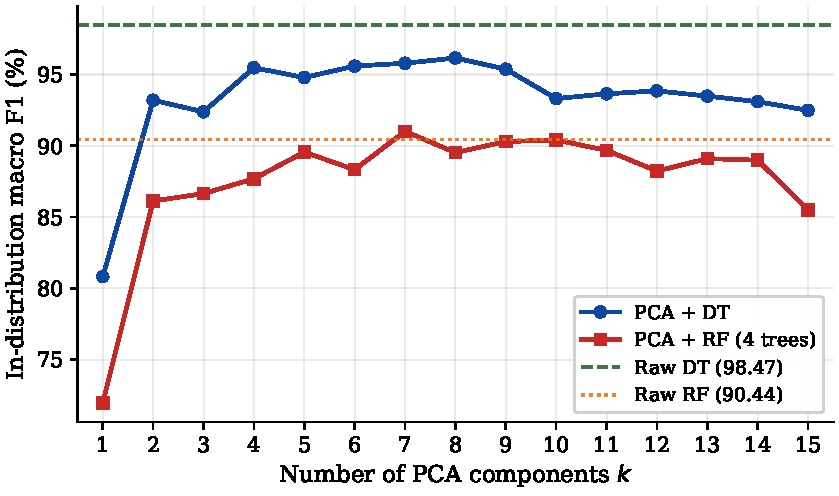
\includegraphics[width=0.75\textwidth]{images/fig_acc_vs_k.pdf}
    \caption{In-distribution macro F1 versus the number of PCA components $k$, on the CIC-IoT 2023 test partition.}
    \label{fig:acc_vs_k}
\end{figure}

The macro F1 aggregates four distinct per-class behaviors; Fig.~\ref{fig:perclass_indist} therefore reports per-class F1 for the DT and RF families. The raw DT approaches saturation on every attack class (BruteForce $99.07\%$, DoS $99.57\%$, Reconnaissance $99.51\%$) with Benign at $95.72\%$, so the reduction from PCA is not a per-class collapse but a roughly uniform decrease as $k$ varies. PCA $+$ DT recovers substantially: BruteForce and DoS exceed $97\%$ at $k{=}5$ and Reconnaissance reaches $95.31\%$ at the same $k$. PCA $+$ RF performs poorly on Reconnaissance, where its best F1 across $k\!\in\!\{1,\dots,15\}$ is $79.61\%$, because the four-tree majority vote misclassifies rare scanning patterns as neighboring benign codes once the feature space is compressed.

\begin{figure}[!t]
    \centering
    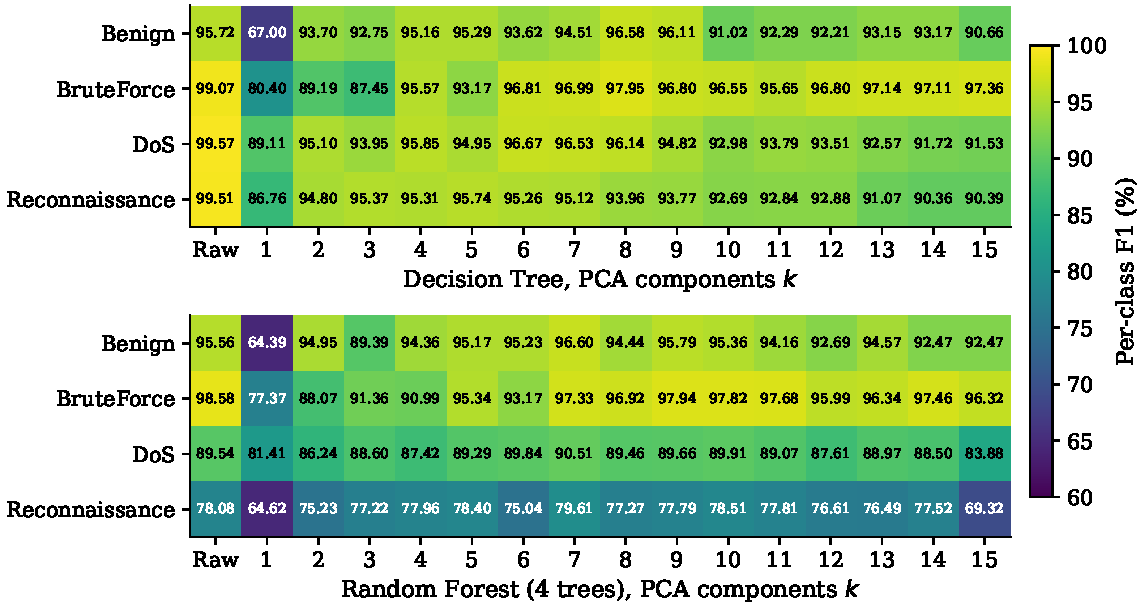
\includegraphics[width=0.95\textwidth]{images/fig_perclass_indist.pdf}
    \caption{Per-class F1 on the CIC-IoT 2023 test partition for the Decision Tree (top) and the 4-tree Random Forest (bottom). The first column ($k{=}\mathrm{Raw}$) is the no-PCA baseline; the remaining columns are PCA settings $k\!\in\!\{1,\dots,15\}$.}
    \label{fig:perclass_indist}
\end{figure}

The P4 footprint of the PCA configurations is dominated by the additive PCA transform tables. Total table entries stay between $10\,200$ and $11\,000$ for every $k\!\in\!\{2,\dots,15\}$, against $5\,119$ for the raw DT and $6\,769$ for the raw RF (Fig.~\ref{fig:p4_footprint}, right). The PCA $+$ DT footprint is therefore about twice the raw DT footprint, and the PCA $+$ RF footprint is about $1.6$ times the raw RF baseline. The relative overhead of adding the projection stage is therefore moderate and decreases for the RF family, where the per-tree classifier tables already account for a larger share of the entry budget. The classifier match-key grows linearly with $k$ at $b{=}32$, from $32$ bits at $k{=}1$ to $480$ bits at $k{=}15$, and equals the raw DT baseline of $256$ bits exactly at $k{=}8$, exceeding it for $k\!\geq\!9$ (Fig.~\ref{fig:p4_footprint}, left). PCA therefore narrows the match-key for $k\!\leq\!7$ and widens it for $k\!\geq\!9$, so the recommended operating point at $k{=}7$ yields a narrower key than the raw DT baseline.

\begin{figure}[!t]
    \centering
    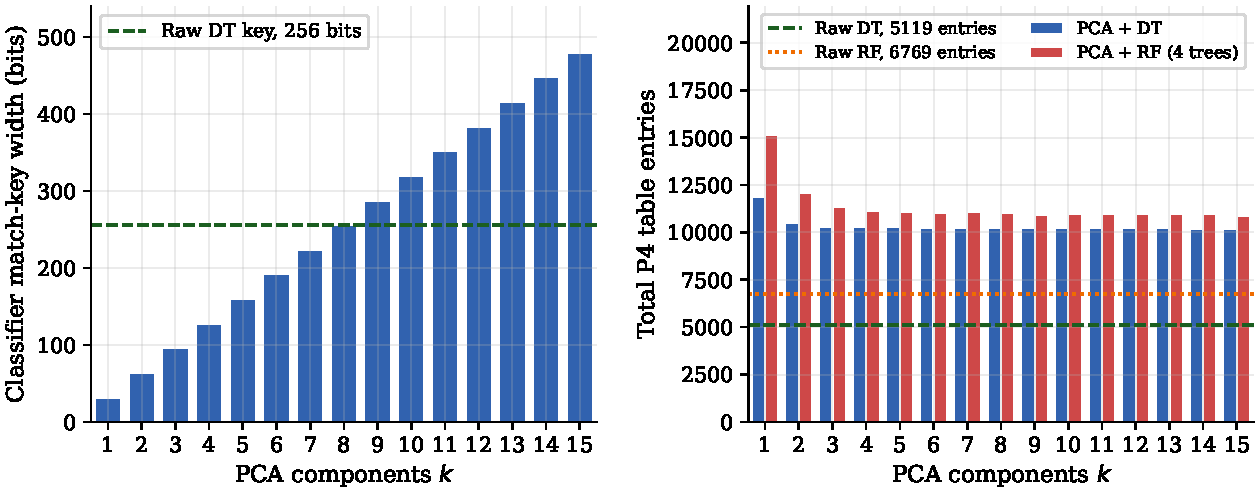
\includegraphics[width=0.95\textwidth]{images/fig_p4_footprint.pdf}
    \caption{Classifier match-key width (left) and total P4 table entries (right) versus the number of PCA components $k$.}
    \label{fig:p4_footprint}
\end{figure}

Under cross-dataset evaluation, the same trained models process the disjoint Mu-IoT capture through the identical pipeline without any retraining. The raw DT degrades from $98.47\%$ macro F1 in distribution to $15.57\%$ on Mu-IoT, while PCA $+$ DT in the $k\!\in\!\{4,\dots,8\}$ band sustains $44.68\%$ to $48.31\%$ (Fig.~\ref{fig:xds_overall}), a gain of $29$ to $33$ percentage points. The improvement is attributable primarily to DoS detection: the raw DT fails to transfer DoS because the CIC-IoT DoS class is concentrated on a single destination port absent from the Mu-IoT testbed, while the additive PCA projection combines the $18$ features into composite components before quantization, breaking the classifier's dependence on any single feature and producing multi-feature combinations whose decision boundaries prove more stable under distribution shift.

\begin{figure}[!t]
    \centering
    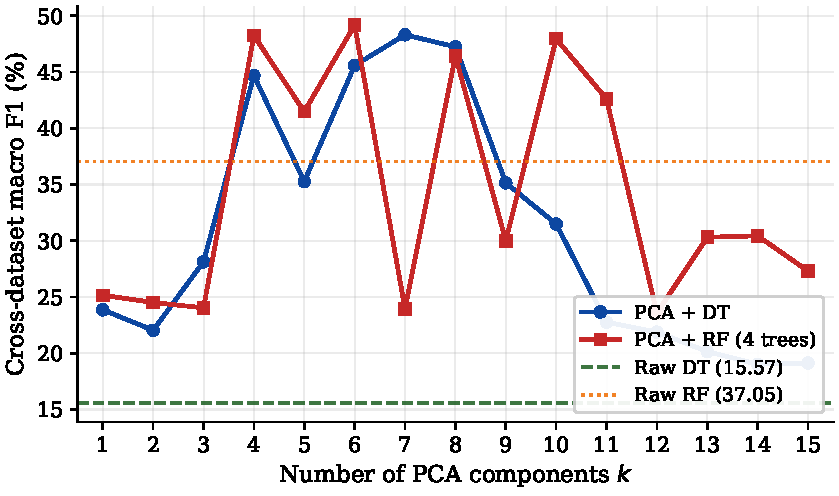
\includegraphics[width=0.75\textwidth]{images/fig_xds_overall.pdf}
    \caption{Cross-dataset macro F1 on the Mu-IoT testbed versus the number of PCA components $k$.}
    \label{fig:xds_overall}
\end{figure}

The two regimes prefer different pipelines, so the deployable operating point is selected through the standard Pareto-efficiency criterion~\cite{Pareto1906,MarlerArora2004}: a configuration is Pareto-efficient when no other configuration improves it on every objective simultaneously, with in-distribution macro F1 and cross-dataset macro F1 as the two objectives. Fig.~\ref{fig:pareto} plots all $32$ configurations; four lie on the Pareto front: raw DT ($98.47\%$, $15.57\%$), PCA $+$ DT at $k{=}8$ ($96.16\%$, $47.24\%$), PCA $+$ DT at $k{=}7$ ($95.79\%$, $48.31\%$), and PCA $+$ RF at $k{=}6$ ($88.32\%$, $49.18\%$). PCA $+$ DT at $k{=}7$ is the recommended operating point: it achieves the highest cross-dataset F1 among DT-family Pareto configurations ($48.31\%$ versus $47.24\%$ at $k{=}8$), so $k{=}8$ trades $1.07$ percentage points of cross-dataset performance for only $0.37$ percentage points more in-distribution — an unfavourable exchange for deployment. The only Pareto configuration with higher cross-dataset F1 is PCA $+$ RF at $k{=}6$ ($49.18\%$), but its $0.87$ percentage-point cross-dataset advantage comes at the cost of $7.47$ percentage points of in-distribution F1 ($88.32\%$ versus $95.79\%$). Additionally, $k{=}7$ has a narrower classifier key than $k{=}8$ ($224$ versus $256$ bits). Table~\ref{tab:vs_raw} summarizes this operating point against the raw DT baseline.

\begin{figure}[!t]
    \centering
    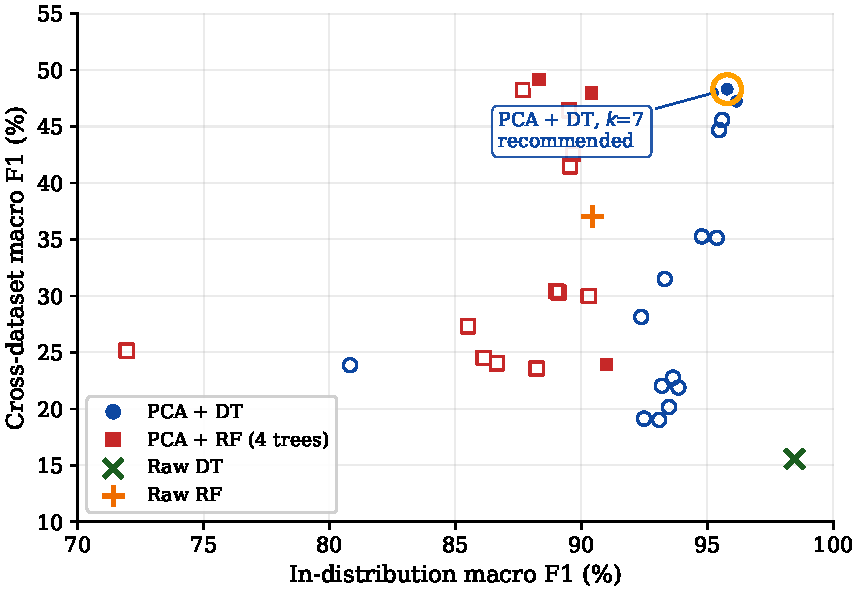
\includegraphics[width=0.75\textwidth]{images/fig_pareto.pdf}
    \caption{Configurations plotted on the two objective axes used for operating-point selection: in-distribution macro F1 (CIC-IoT 2023) on the $x$ axis and cross-dataset macro F1 (Mu-IoT testbed) on the $y$ axis. Filled markers lie on the Pareto front; the highlighted point is the recommended PCA $+$ DT at $k{=}7$.}
    \label{fig:pareto}
\end{figure}

\begin{table}[t]
\centering
\setlength{\tabcolsep}{4pt}
\caption{Recommended PCA $+$ DT operating point ($k{=}7$, $b{=}32$) compared with the raw range-match DT baseline. All figures are measured on the Raspberry Pi~4 testbed on the CIC-IoT 2023 test partition and the Mu-IoT cross-dataset capture.}
\label{tab:vs_raw}
\begin{tabular}{l r r l}
\toprule
\textbf{Metric} & \textbf{Raw DT} & \textbf{PCA $+$ DT} & \textbf{Winner} \\
\midrule
P4 entries (total)        & $5\,119$       & $10\,222$    & Raw (about $2$ times fewer) \\
Classifier key (bits)     & $256$       & $224$        & PCA ($12.50\%$ narrower) \\
Rules-load time           & $10.09$ s   & $21.55$ s    & Raw \\
In-distribution macro F1  & $98.47\%$   & $95.79\%$    & Raw ($+2.68$ pp) \\
Cross-dataset macro F1    & $15.57\%$   & $48.31\%$    & PCA ($+32.74$ pp) \\
\bottomrule
\end{tabular}
\end{table}

%──────────────────────────────────────────────────────────────────────
\section{Towards Hardware Deployment on Intel Tofino}\label{sec:tofino}
%──────────────────────────────────────────────────────────────────────

The measurements in Section~\ref{sec:results} are collected on a Raspberry Pi~4 running BMv2, which executes the v1model pipeline in software. Deploying the same design on an ASIC such as Intel Tofino is necessary for higher-tier IoT and cyber-physical workloads but imposes strict constraints on pipeline depth, on-chip memory, match resources, and action complexity~\cite{Bosshart2013}. The hardware pressure of the proposed pipeline comes from three sources: stateful flow storage in the feature-accumulation block (SRAM scales with the number of tracked flows times the per-flow register footprint), match-action resources in the PCA transform and classifier (range tables compile to TCAM, bounded by entry count and match-key width), and control-plane reporting via Tofino digests (triggered event-driven on flow termination, idle timeout, or attack classification rather than per packet).

The raw range-match DT keys on an $18$-feature composite vector of $256$ bits (Table~\ref{tab:features}); the recommended PCA $+$ DT at $k{=}7$ keys on $224$ bits. Both are within the match-key width supported per stage by an RMT-style pipeline~\cite{Bosshart2013}, of which Tofino-1 is the production instance, so match-key width is not the binding constraint and no key-width reduction is required. To make the per-stage allocation concrete, Table~\ref{tab:feature_bits} proposes a Tofino-friendly grouping of the deployed $18$ features into eight $32$-bit PHV slots: each row represents one $32$-bit slot holding two $16$-bit fields (or four $8$-bit fields in the case of the flag pairs in row~1), and the eight slots together total $256$ bits, matching the BMv2 raw composite key without any additional widening introduced by the ASIC layout. The grouping is illustrative rather than measured: porting the design to Tofino has not yet been performed.

\begin{table}[t]
\centering
\setlength{\tabcolsep}{4pt}
\renewcommand{\arraystretch}{1.0}
\caption{Illustrative grouping of the $18$ deployed features into eight $32$-bit PHV slots for a Tofino port. Each row represents one $32$-bit slot containing two $16$-bit fields (row~1 instead packs four $8$-bit flag counters). The total is $256$ bits, the same as the BMv2 raw classifier key.}
\label{tab:feature_bits}
\begin{tabular}{lcclc}
\toprule
\textbf{Field 1} & \textbf{Bits} & \textbf{Container} & \textbf{Field 2} & \textbf{Bits} \\
\midrule
\textit{Protocol} + \textit{FlagsSyn}        & $8 + 8$  & 32-bit & \textit{FlagsFin} + \textit{FlagsRst} & $8 + 8$ \\
\textit{SrcPort}                             & $16$     & 32-bit & \textit{DstPort}                      & $16$ \\
\textit{Duration}                            & $16$     & 32-bit & \textit{MaxIAT}                       & $16$ \\
\textit{FwdPktCount}                         & $16$     & 32-bit & \textit{BwdPktCount}                  & $16$ \\
\textit{FwdBytes}                            & $16$     & 32-bit & \textit{BwdBytes}                     & $16$ \\
\textit{FwdMaxPktLen}                        & $16$     & 32-bit & \textit{BwdMaxPktLen}                 & $16$ \\
\textit{FlagsAck}                            & $16$     & 32-bit & \textit{FlagsPsh}                     & $16$ \\
\textit{MaxWinSize}                          & $16$     & 32-bit & \textit{InitFwdWinBytes}              & $16$ \\
\midrule
\multicolumn{4}{l}{\textbf{Total}}                                                          & $\mathbf{256}$ \\
\bottomrule
\end{tabular}
\end{table}

The binding constraint is therefore pipeline depth, not match-key width. An offline estimator that counts one stage per major data-dependent operation reports: $18$ stages for feature extraction (one register read-write per bidirectional feature), one stage for quantization, $k$ stages for the additive PCA transform (one per component), and one stage for the classifier, totalling $20$ stages for the raw DT and $21$ to $35$ stages for PCA configurations ($k{=}1$ to $k{=}15$), against the $12$-stage Tofino-1 ingress budget. Stage-count compaction is therefore the central hardware engineering task for the Tofino port, with the following three concrete directions identified. First, tighter feature selection retains fewer but more informative inputs, shrinking the feature-accumulation block and its stage count proportionally. Second, conditional shared-stage placement of the per-flow register arrays uses a single stateful ALU action that branches on the direction bit to update either the forward or the backward counter within one stage, rather than two separate stages. Third, multiple per-feature contribution range-match lookups are combined into compound tables with joint keys, resolving two or more features in a single stage at the cost of larger table entries. These directions are the subject of future work targeting the UfiSpace S9180-32X / BFN-T10-032D Tofino testbed.

%──────────────────────────────────────────────────────────────────────
\section{Conclusion and Future Work}\label{sec:cons}
%──────────────────────────────────────────────────────────────────────

This paper has presented an automated pipeline for tree-based multiclass IoT attack detection entirely inside a P4 data plane. The classifier is encoded on $18$ bidirectional flow features as a range-match table with one entry per tree leaf, and an optional additive PCA stage is itself encoded as one single-field range table per input feature. Across $32$ configurations deployed on a Raspberry Pi~4, the in-distribution and cross-dataset regimes prefer different pipelines. In distribution on CIC-IoT 2023 the raw DT achieves the highest macro F1 ($98.47\%$, $5\,119$ entries, $256$-bit key); on the disjoint Mu-IoT capture it degrades to $15.57\%$ because the model fails to generalize to the new traffic distribution. PCA + DT at $k{=}7$ trades $2.68$ percentage points of in-distribution macro F1 ($95.79\%$, $10\,222$ entries) for a $+32.74$ percentage-point gain in cross-dataset macro F1 ($48.31\%$), and is therefore the recommended deployable operating point. A Tofino-1 resource analysis confirms that both pipelines fit the per-stage match-key budget; stage-count compaction through the directions described in Section~\ref{sec:tofino} is the identified path to full ASIC deployment. Future work will validate the pipeline on a Tofino testbed, extend the cross-dataset evaluation to UNSW-NB15, CIC-IDS 2017, and EDGE-IIoTset, and add controller-driven incremental rule updates.

\begin{credits}
\subsubsection{\ackname} This work was supported by the Ministry of Industry and Trade of the Czech Republic under Grant No.~CZ.01.01.01/01/24\_062/0007470. It was also funded in part by the German Research Foundation (DFG, Deutsche Forschungsgemeinschaft) under Germany’s Excellence Strategy-EXC 2050/2, Project ID 390696704 (Cluster of Excellence “Centre for Tactile Internet with Human-in-the-Loop” (CeTI), TU Dresden), and by the Federal Ministry of Education and Research of Germany in the programme of "Souverän. Digital. Vernetzt.". Joint project 6G-life, project identification number: 16KIS2413K.
\end{credits}

\bibliographystyle{splncs04}
\bibliography{references}

\end{document}